\section{Second order differential equations}
In this section, we will learn how to solve second order ODEs with constant coefficients. These are ODEs of the form

\[y'' + Ay' + By = f(x)\] or \[\frac{d^2y}{dx^2} + A\frac{dy}{dx} + By = f(x)\] where \(A,B\in\mathbb{R}\).

To solve equations like this, we look for particular integrals and complementary functions to make solutions of the form:
\[y(x)=\underbrace{f(x)}_{\text{particular integral (P.I.)}}+\underbrace{Cg(x)}_{\text{complementary function (C.F.)}},\]

\subsection{Finding complementary functions}
In this section we will be looking for solutions of the homogenous ODE \[\frac{d^2y}{dx^2} + A\frac{dy}{dx} + By = 0.\]
These will be the complementary functions of the non-homogenous ODE.
\begin{definition}
Two functions, $y_1$ and $y_2$ are \textbf{independent} if one is not a multiple of the other; otherwise, they are said to be \textbf{dependent}.
\end{definition}

\begin{example}
$y_1(x)=1$ and $y_2(x)=x$ are independent.

$y_1(x)=x$ and $y_2(x)=3x$ are dependent because $y_2(x)=3y_1(x)$.

$y_1(x)=e^{ax}$ and $y_2(x)=e^{bx}$ ($a\ne b$) are independent.
\end{example}

\begin{theorem}
If $y_1(x)$ and $y_2(x)$ are independent and they are the solutions to
\[\frac{d^2y}{dx^2} + A\frac{dy}{dx} + By = 0\]
 then the complementary function of this ODE is
\[y(x)=c_1y_1(x)+c_2y_2(x),\]
where $c_1$ and $c_2$ are constants.

In other words, if you have two independent solutions to the homogenous equation, then you can represent any other solution to the homogenous
equation in terms of these two solutions.
\end{theorem}

Therefore our aim is to find two independent solutions to 
\[\frac{d^2y}{dx^2} + A\frac{dy}{dx} + By = 0\]
If we look for solutions of the form
\[y=e^{\lambda x},\]
then
\[y'=\lambda e^{\lambda x},\quad y''=\lambda^2e^{\lambda x},\]
and so
\begin{align*}
y''+Ay'+By&=\lambda^2e^{\lambda x}+A\lambda e^{\lambda x}+Be^{\lambda x}\\&=e^{\lambda x}(\lambda^2+A\lambda+B).
\end{align*}
Therefore
\[e^{\lambda x}(\lambda^2+A\lambda+B)\equiv0.\]
This will be zero when
\[\lambda^2+A\lambda+B=0\]

\begin{definition}
\[\lambda^2+A\lambda+B=0\] is called the \textbf{characteristic equation} or \textbf{auxiliary equation} of the ODE \[\frac{d^2y}{dx^2} + A\frac{dy}{dx} + By = 0.\]
\end{definition}

In general, we know that the roots of the auxiliary equation are given by
\[\lambda = \frac{-A\pm\sqrt{A^2-4B}}{2}\]
There are three cases, depending on the value of $\Delta=A^2-4B$.
\begin{figure}[H]
    \hspace{0.2cm}
    \subfigure[Two roots]{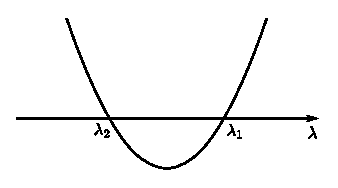
\includegraphics[scale=0.75]{img/lam-two-roots}}
    \hspace{0.5cm}
    \subfigure[One root]{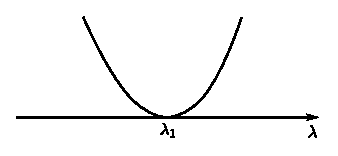
\includegraphics[scale=0.75]{img/lam-one-root}}
        \hspace{0.5cm}
    \subfigure[No roots (complex)]{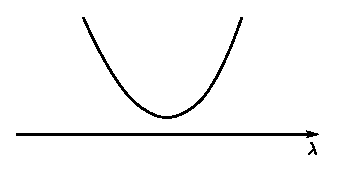
\includegraphics[scale=0.75]{img/lam-no-roots}} \\
    \centering
  \caption{Different options for the curve $y=\lambda^2+A\lambda+B$ when solving the equation $\lambda^2+A\lambda+B=0$.}
\end{figure}

\subsubsection{Case 1: $\Delta>0$}
If $\Delta>0$, we have two distinct real roots:
\[\lambda_1=\frac{-r+\sqrt{\Delta}}{2}\quad\text{ and }\quad \lambda_2=\frac{-r-\sqrt{\Delta}}{2}\]

The general solution to the homogenous equation is 
\[g(x)=C_1e^{\lambda_1x}+C_2e^{\lambda_2x}.\]

\begin{example}
Consider the second order differential equation
\[y''+3y'+2y=0.\]
The auxiliary equation is
\[\lambda^2+3\lambda+2=0\]
\[(\lambda+1)(\lambda+2)=0.\]
This has two roots:
\[\lambda_1=-1,\quad \lambda_2=-2.\]
Therefore we have two solutions $e^{-x}$ and $e^{-2x}$, and they are independent. So the general solution is
\[y(x)=c_1e^{-x}+c_2e^{-2x}.\]
\end{example}

\subsubsection{Case 2: $\Delta=0$}
If $\Delta=0$, the auxiliary equation has one root which is real, given by
\[\lambda_1=\frac{A}{B}.\]

So $e^{\lambda_1x}$ is one solution to the homogenous equation. We need to find another solution, which is independent of $e^{\lambda_1x}$. So we try
\[y_2(x)=xe^{\lambda_1x}.\]

\[y'=e^{\lambda_1 x}+\lambda_1xe^{\lambda_1x}\]
\begin{align*}
y''&=\lambda_1e^{\lambda_1 x}+\lambda_1e^{\lambda_1 x}+\lambda_1^2xe^{\lambda_1 x}\\
&=\lambda_1^2xe^{\lambda_1 x}+2\lambda_1e^{\lambda_1 x}.
\end{align*}

Therefore
\begin{align*}
y''+Ay'+By &= \lambda_1^2xe^{\lambda_1 x}+2\lambda_1e^{\lambda_1 x}+Ae^{\lambda_1 x}+A\lambda_1xe^{\lambda_1x}+Bxe^{\lambda_1x} \\
&= \underbrace{(\lambda_1^2+A\lambda_1+B)}_{=0}xe^{\lambda_1x} + \underbrace{(2\lambda_1 +A)}_{=0}e^{\lambda_1x} \\
&= 0.
\end{align*}
Therefore, $xe^{\lambda_1x}$ is the second independent solution. Thereforre, the general solution of the homogenous equation is
\[g(x)=c_1e^{\lambda_1x}+c_2xe^{\lambda_1x}\]
or
\[g(x)=(c_1+c_2x)e^{\lambda_1x}.\]

\begin{example}
Consider the differential equation
\[y''+2y'+y=0.\]
The auxiliary equation is:
\[\lambda^2+2\lambda+1=0\]\[(\lambda+1)^2=0\]\[\lambda_1=-1\]
$\lambda_1$ is the only root.

$e^{\lambda_1x}$ and $xe^{\lambda_1x}$ are two independent solutions, so the general solution is
\[y(x)=c_1e^{-x}+c_2xe^{-x}\] or \[y(x)=e^{-x}(c_1+c_2x).\]
\end{example}

\subsubsection{Case 3: $\Delta<0$}
If $\Delta<0$, there is no real solution to the auxiliary equation.
But it is still possible to find two independent solutions, which give the general solution
\[g(x)=e^{\alpha x}\left( c_1\cos \beta x + c_2\sin \beta x \right),\]
where \[\alpha=-\frac{A}{2}\] and \[\beta=\frac{\sqrt{4B-A^2}}{2}.\]

Complex numbers can be used to show that these are the solutions.\footnote{Details of how this is done can be found on Moodle or at \url{http://www.mscroggs.co.uk/6103}.}

\begin{example}
Consider the differential equation
\[y''-6y'+13y=0.\]
The auxiliary equation is
\[\lambda^2-6\lambda +13=0,\]
which has 
\[A=-6,\quad B=13,\quad \Delta=A^2-Bs=36-52=-16<0,\]
i.e. it has complex roots. So we have
\[\alpha=-\frac{-6}{2}=3,\quad \beta=\frac{1}{2}\sqrt{4\cdot13-(-6)^2}=2,\]
therefore $e^{3x}\cos 2x$ and $e^{3x}\sin 2x$ are two independent solutions, so
\[y=e^{3x}(c_1\cos 2x + c_2\sin 2x),\]
is the general solution.
\end{example}
